%% bare_jrnl.tex
%% V1.4b
%% 2015/08/26
%% by Michael Shell
%% see http://www.michaelshell.org/
%% for current contact information.
%%
%% This is a skeleton file demonstrating the use of IEEEtran.cls
%% (requires IEEEtran.cls version 1.8b or later) with an IEEE
%% journal paper.
%%
%% Support sites:
%% http://www.michaelshell.org/tex/ieeetran/
%% http://www.ctan.org/pkg/ieeetran
%% and
%% http://www.ieee.org/

%%*************************************************************************
%% Legal Notice:
%% This code is offered as-is without any warranty either expressed or
%% implied; without even the implied warranty of MERCHANTABILITY or
%% FITNESS FOR A PARTICULAR PURPOSE! 
%% User assumes all risk.
%% In no event shall the IEEE or any contributor to this code be liable for
%% any damages or losses, including, but not limited to, incidental,
%% consequential, or any other damages, resulting from the use or misuse
%% of any information contained here.
%%
%% All comments are the opinions of their respective authors and are not
%% necessarily endorsed by the IEEE.
%%
%% This work is distributed under the LaTeX Project Public License (LPPL)
%% ( http://www.latex-project.org/ ) version 1.3, and may be freely used,
%% distributed and modified. A copy of the LPPL, version 1.3, is included
%% in the base LaTeX documentation of all distributions of LaTeX released
%% 2003/12/01 or later.
%% Retain all contribution notices and credits.
%% ** Modified files should be clearly indicated as such, including  **
%% ** renaming them and changing author support contact information. **
%%*************************************************************************


% *** Authors should verify (and, if needed, correct) their LaTeX system  ***
% *** with the testflow diagnostic prior to trusting their LaTeX platform ***
% *** with production work. The IEEE's font choices and paper sizes can   ***
% *** trigger bugs that do not appear when using other class files.       ***                          ***
% The testflow support page is at:
% http://www.michaelshell.org/tex/testflow/



\documentclass[journal]{IEEEtran}
%
% If IEEEtran.cls has not been installed into the LaTeX system files,
% manually specify the path to it like:
% \documentclass[journal]{../sty/IEEEtran}





% Some very useful LaTeX packages include:
% (uncomment the ones you want to load)


% *** MISC UTILITY PACKAGES ***
%
%\usepackage{ifpdf}
% Heiko Oberdiek's ifpdf.sty is very useful if you need conditional
% compilation based on whether the output is pdf or dvi.
% usage:
% \ifpdf
%   % pdf code
% \else
%   % dvi code
% \fi
% The latest version of ifpdf.sty can be obtained from:
% http://www.ctan.org/pkg/ifpdf
% Also, note that IEEEtran.cls V1.7 and later provides a builtin
% \ifCLASSINFOpdf conditional that works the same way.
% When switching from latex to pdflatex and vice-versa, the compiler may
% have to be run twice to clear warning/error messages.






% *** CITATION PACKAGES ***
%
%\usepackage{cite}
% cite.sty was written by Donald Arseneau
% V1.6 and later of IEEEtran pre-defines the format of the cite.sty package
% \cite{} output to follow that of the IEEE. Loading the cite package will
% result in citation numbers being automatically sorted and properly
% "compressed/ranged". e.g., [1], [9], [2], [7], [5], [6] without using
% cite.sty will become [1], [2], [5]--[7], [9] using cite.sty. cite.sty's
% \cite will automatically add leading space, if needed. Use cite.sty's
% noadjust option (cite.sty V3.8 and later) if you want to turn this off
% such as if a citation ever needs to be enclosed in parenthesis.
% cite.sty is already installed on most LaTeX systems. Be sure and use
% version 5.0 (2009-03-20) and later if using hyperref.sty.
% The latest version can be obtained at:
% http://www.ctan.org/pkg/cite
% The documentation is contained in the cite.sty file itself.






% *** GRAPHICS RELATED PACKAGES ***
%
\ifCLASSINFOpdf
  % \usepackage[pdftex]{graphicx}
  % declare the path(s) where your graphic files are
  % \graphicspath{{../pdf/}{../jpeg/}}
  % and their extensions so you won't have to specify these with
  % every instance of \includegraphics
  % \DeclareGraphicsExtensions{.pdf,.jpeg,.png}
\else
  % or other class option (dvipsone, dvipdf, if not using dvips). graphicx
  % will default to the driver specified in the system graphics.cfg if no
  % driver is specified.
  % \usepackage[dvips]{graphicx}
  % declare the path(s) where your graphic files are
  % \graphicspath{{../eps/}}
  % and their extensions so you won't have to specify these with
  % every instance of \includegraphics
  % \DeclareGraphicsExtensions{.eps}
\fi
% graphicx was written by David Carlisle and Sebastian Rahtz. It is
% required if you want graphics, photos, etc. graphicx.sty is already
% installed on most LaTeX systems. The latest version and documentation
% can be obtained at: 
% http://www.ctan.org/pkg/graphicx
% Another good source of documentation is "Using Imported Graphics in
% LaTeX2e" by Keith Reckdahl which can be found at:
% http://www.ctan.org/pkg/epslatex
%
% latex, and pdflatex in dvi mode, support graphics in encapsulated
% postscript (.eps) format. pdflatex in pdf mode supports graphics
% in .pdf, .jpeg, .png and .mps (metapost) formats. Users should ensure
% that all non-photo figures use a vector format (.eps, .pdf, .mps) and
% not a bitmapped formats (.jpeg, .png). The IEEE frowns on bitmapped formats
% which can result in "jaggedy"/blurry rendering of lines and letters as
% well as large increases in file sizes.
%
% You can find documentation about the pdfTeX application at:
% http://www.tug.org/applications/pdftex

\usepackage{amsmath}
\usepackage{subfig}
\usepackage{booktabs}
\usepackage{graphicx}
\usepackage{caption}
\usepackage{pgfplots}
\usetikzlibrary{pgfplots.groupplots}
\graphicspath{ {./imgs/} }


% *** MATH PACKAGES ***
%
%\usepackage{amsmath}
% A popular package from the American Mathematical Society that provides
% many useful and powerful commands for dealing with mathematics.
%
% Note that the amsmath package sets \interdisplaylinepenalty to 10000
% thus preventing page breaks from occurring within multiline equations. Use:
%\interdisplaylinepenalty=2500
% after loading amsmath to restore such page breaks as IEEEtran.cls normally
% does. amsmath.sty is already installed on most LaTeX systems. The latest
% version and documentation can be obtained at:
% http://www.ctan.org/pkg/amsmath





% *** SPECIALIZED LIST PACKAGES ***
%
%\usepackage{algorithmic}
% algorithmic.sty was written by Peter Williams and Rogerio Brito.
% This package provides an algorithmic environment fo describing algorithms.
% You can use the algorithmic environment in-text or within a figure
% environment to provide for a floating algorithm. Do NOT use the algorithm
% floating environment provided by algorithm.sty (by the same authors) or
% algorithm2e.sty (by Christophe Fiorio) as the IEEE does not use dedicated
% algorithm float types and packages that provide these will not provide
% correct IEEE style captions. The latest version and documentation of
% algorithmic.sty can be obtained at:
% http://www.ctan.org/pkg/algorithms
% Also of interest may be the (relatively newer and more customizable)
% algorithmicx.sty package by Szasz Janos:
% http://www.ctan.org/pkg/algorithmicx




% *** ALIGNMENT PACKAGES ***
%
%\usepackage{array}
% Frank Mittelbach's and David Carlisle's array.sty patches and improves
% the standard LaTeX2e array and tabular environments to provide better
% appearance and additional user controls. As the default LaTeX2e table
% generation code is lacking to the point of almost being broken with
% respect to the quality of the end results, all users are strongly
% advised to use an enhanced (at the very least that provided by array.sty)
% set of table tools. array.sty is already installed on most systems. The
% latest version and documentation can be obtained at:
% http://www.ctan.org/pkg/array


% IEEEtran contains the IEEEeqnarray family of commands that can be used to
% generate multiline equations as well as matrices, tables, etc., of high
% quality.




% *** SUBFIGURE PACKAGES ***
%\ifCLASSOPTIONcompsoc
%  \usepackage[caption=false,font=normalsize,labelfont=sf,textfont=sf]{subfig}
%\else
%  \usepackage[caption=false,font=footnotesize]{subfig}
%\fi
% subfig.sty, written by Steven Douglas Cochran, is the modern replacement
% for subfigure.sty, the latter of which is no longer maintained and is
% incompatible with some LaTeX packages including fixltx2e. However,
% subfig.sty requires and automatically loads Axel Sommerfeldt's caption.sty
% which will override IEEEtran.cls' handling of captions and this will result
% in non-IEEE style figure/table captions. To prevent this problem, be sure
% and invoke subfig.sty's "caption=false" package option (available since
% subfig.sty version 1.3, 2005/06/28) as this is will preserve IEEEtran.cls
% handling of captions.
% Note that the Computer Society format requires a larger sans serif font
% than the serif footnote size font used in traditional IEEE formatting
% and thus the need to invoke different subfig.sty package options depending
% on whether compsoc mode has been enabled.
%
% The latest version and documentation of subfig.sty can be obtained at:
% http://www.ctan.org/pkg/subfig




% *** FLOAT PACKAGES ***
%
%\usepackage{fixltx2e}
% fixltx2e, the successor to the earlier fix2col.sty, was written by
% Frank Mittelbach and David Carlisle. This package corrects a few problems
% in the LaTeX2e kernel, the most notable of which is that in current
% LaTeX2e releases, the ordering of single and double column floats is not
% guaranteed to be preserved. Thus, an unpatched LaTeX2e can allow a
% single column figure to be placed prior to an earlier double column
% figure.
% Be aware that LaTeX2e kernels dated 2015 and later have fixltx2e.sty's
% corrections already built into the system in which case a warning will
% be issued if an attempt is made to load fixltx2e.sty as it is no longer
% needed.
% The latest version and documentation can be found at:
% http://www.ctan.org/pkg/fixltx2e


%\usepackage{stfloats}
% stfloats.sty was written by Sigitas Tolusis. This package gives LaTeX2e
% the ability to do double column floats at the bottom of the page as well
% as the top. (e.g., "\begin{figure*}[!b]" is not normally possible in
% LaTeX2e). It also provides a command:
%\fnbelowfloat
% to enable the placement of footnotes below bottom floats (the standard
% LaTeX2e kernel puts them above bottom floats). This is an invasive package
% which rewrites many portions of the LaTeX2e float routines. It may not work
% with other packages that modify the LaTeX2e float routines. The latest
% version and documentation can be obtained at:
% http://www.ctan.org/pkg/stfloats
% Do not use the stfloats baselinefloat ability as the IEEE does not allow
% \baselineskip to stretch. Authors submitting work to the IEEE should note
% that the IEEE rarely uses double column equations and that authors should try
% to avoid such use. Do not be tempted to use the cuted.sty or midfloat.sty
% packages (also by Sigitas Tolusis) as the IEEE does not format its papers in
% such ways.
% Do not attempt to use stfloats with fixltx2e as they are incompatible.
% Instead, use Morten Hogholm'a dblfloatfix which combines the features
% of both fixltx2e and stfloats:
%
% \usepackage{dblfloatfix}
% The latest version can be found at:
% http://www.ctan.org/pkg/dblfloatfix




%\ifCLASSOPTIONcaptionsoff
%  \usepackage[nomarkers]{endfloat}
% \let\MYoriglatexcaption\caption
% \renewcommand{\caption}[2][\relax]{\MYoriglatexcaption[#2]{#2}}
%\fi
% endfloat.sty was written by James Darrell McCauley, Jeff Goldberg and 
% Axel Sommerfeldt. This package may be useful when used in conjunction with 
% IEEEtran.cls'  captionsoff option. Some IEEE journals/societies require that
% submissions have lists of figures/tables at the end of the paper and that
% figures/tables without any captions are placed on a page by themselves at
% the end of the document. If needed, the draftcls IEEEtran class option or
% \CLASSINPUTbaselinestretch interface can be used to increase the line
% spacing as well. Be sure and use the nomarkers option of endfloat to
% prevent endfloat from "marking" where the figures would have been placed
% in the text. The two hack lines of code above are a slight modification of
% that suggested by in the endfloat docs (section 8.4.1) to ensure that
% the full captions always appear in the list of figures/tables - even if
% the user used the short optional argument of \caption[]{}.
% IEEE papers do not typically make use of \caption[]'s optional argument,
% so this should not be an issue. A similar trick can be used to disable
% captions of packages such as subfig.sty that lack options to turn off
% the subcaptions:
% For subfig.sty:
% \let\MYorigsubfloat\subfloat
% \renewcommand{\subfloat}[2][\relax]{\MYorigsubfloat[]{#2}}
% However, the above trick will not work if both optional arguments of
% the \subfloat command are used. Furthermore, there needs to be a
% description of each subfigure *somewhere* and endfloat does not add
% subfigure captions to its list of figures. Thus, the best approach is to
% avoid the use of subfigure captions (many IEEE journals avoid them anyway)
% and instead reference/explain all the subfigures within the main caption.
% The latest version of endfloat.sty and its documentation can obtained at:
% http://www.ctan.org/pkg/endfloat
%
% The IEEEtran \ifCLASSOPTIONcaptionsoff conditional can also be used
% later in the document, say, to conditionally put the References on a 
% page by themselves.




% *** PDF, URL AND HYPERLINK PACKAGES ***
%
%\usepackage{url}
% url.sty was written by Donald Arseneau. It provides better support for
% handling and breaking URLs. url.sty is already installed on most LaTeX
% systems. The latest version and documentation can be obtained at:
% http://www.ctan.org/pkg/url
% Basically, \url{my_url_here}.




% *** Do not adjust lengths that control margins, column widths, etc. ***
% *** Do not use packages that alter fonts (such as pslatex).         ***
% There should be no need to do such things with IEEEtran.cls V1.6 and later.
% (Unless specifically asked to do so by the journal or conference you plan
% to submit to, of course. )


% correct bad hyphenation here
\hyphenation{op-tical net-works semi-conduc-tor}


\begin{document}
%
% paper title
% Titles are generally capitalized except for words such as a, an, and, as,
% at, but, by, for, in, nor, of, on, or, the, to and up, which are usually
% not capitalized unless they are the first or last word of the title.
% Linebreaks \\ can be used within to get better formatting as desired.
% Do not put math or special symbols in the title.
\title{A Comparative Study of Genetic-Based Approaches for Enhanced Hourly Temperature Predictions}
%
%
% author names and IEEE memberships
% note positions of commas and nonbreaking spaces ( ~ ) LaTeX will not break
% a structure at a ~ so this keeps an author's name from being broken across
% two lines.
% use \thanks{} to gain access to the first footnote area
% a separate \thanks must be used for each paragraph as LaTeX2e's \thanks
% was not built to handle multiple paragraphs
%

\author{Fabrizio~Sandri\\
University of Trento, Italy}

% note the % following the last \IEEEmembership and also \thanks - 
% these prevent an unwanted space from occurring between the last author name
% and the end of the author line. i.e., if you had this:
% 
% \author{....lastname \thanks{...} \thanks{...} }
%                     ^------------^------------^----Do not want these spaces!
%
% a space would be appended to the last name and could cause every name on that
% line to be shifted left slightly. This is one of those "LaTeX things". For
% instance, "\textbf{A} \textbf{B}" will typeset as "A B" not "AB". To get
% "AB" then you have to do: "\textbf{A}\textbf{B}"
% \thanks is no different in this regard, so shield the last } of each \thanks
% that ends a line with a % and do not let a space in before the next \thanks.
% Spaces after \IEEEmembership other than the last one are OK (and needed) as
% you are supposed to have spaces between the names. For what it is worth,
% this is a minor point as most people would not even notice if the said evil
% space somehow managed to creep in.



% The paper headers
% \markboth{Journal of \LaTeX\ Class Files,~Vol.~14, No.~8, August~2015}%
% {Shell \MakeLowercase{\textit{et al.}}: Bare Demo of IEEEtran.cls for IEEE Journals}
% The only time the second header will appear is for the odd numbered pages
% after the title page when using the twoside option.
% 
% *** Note that you probably will NOT want to include the author's ***
% *** name in the headers of peer review papers.                   ***
% You can use \ifCLASSOPTIONpeerreview for conditional compilation here if
% you desire.




% If you want to put a publisher's ID mark on the page you can do it like
% this:
%\IEEEpubid{0000--0000/00\$00.00~\copyright~2015 IEEE}
% Remember, if you use this you must call \IEEEpubidadjcol in the second
% column for its text to clear the IEEEpubid mark.



% use for special paper notices
%\IEEEspecialpapernotice{(Invited Paper)}




% make the title area
\maketitle

% As a general rule, do not put math, special symbols or citations
% in the abstract or keywords.
\begin{abstract}
Nowadays, time series forecasting is widely applied across various domains. However, addressing the challenges of time series forecasting proves difficult due to factors that extend beyond the data. In this context, approaches based on deep learning and metaheuristics emerge to confront the complexities of time series forecasting by harnessing the inherent data. This study examines two strategies for predicting the outdoor temperature in the upcoming hour: a deep learning model, optimized through Genetic Algorithms, and an interpretable alternative employing Genetic Programming. The analysis aims to compare the results attained through these differing methodologies.

\end{abstract}

% Note that keywords are not normally used for peerreview papers.
\begin{IEEEkeywords}
Time Series Forecasting, Genetic Programming, Genetic Algorithms, LSTM.
\end{IEEEkeywords}






% For peer review papers, you can put extra information on the cover
% page as needed:
% \ifCLASSOPTIONpeerreview
% \begin{center} \bfseries EDICS Category: 3-BBND \end{center}
% \fi
%
% For peerreview papers, this IEEEtran command inserts a page break and
% creates the second title. It will be ignored for other modes.
\IEEEpeerreviewmaketitle


\section{Introduction}
\IEEEPARstart{T}{ime} series forecasting finds its applications across diverse domains, ranging from economic contexts for predicting stock prices to medical scenarios where it aids in forecasting health conditions or diseases over time. Additionally, it plays a crucial role in the realm of weather and climate forecasting, which is the focal point of this study. Specifically, this research delves into utilizing historical data from a weather station to predict future meteorological conditions, particularly the forecast of outdoor weather temperature. The main challenge lies in the amount of factors influencing temperature changes, such as wind, ocean currents, humidity, and other environmental variables. Addressing this problem is challenging not only due to the individual factors but also because of the intricate relationships among them.

In this particular scenario, the adoption of deep learning is deemed appropriate due to its capacity to effectively capture and model intricate relationships inherent in the dataset. The research methodology involves implementing a well-established deep learning model based on recurrent neural networks, with the aim of optimizing its performance by identifying the most suitable hyperparameters through the use of a Genetic Algorithms\cite{genetic-algorithms} for hyperparameter tuning. One notable limitation of deep learning models is their black box nature, where they operate on complex mathematical models that are interpretable only by computers, not humans. Recognizing this lack of interpretability, this study explores an alternative model that can deliver similar results to complex deep neural networks while providing interpretability. This alternative allows for a better understanding of how outputs are derived from inputs, offering transparency in the forecasting process.



\section{Problem Statement}

Consider a weather time series dataset represented as $\{x_1, x_2, \ldots, x_N\}$, where $N$ is the number of samples, and each $x_i$ is a set of relevant features recorded at timestep $i$. The goal is to develop a model that can estimate the outdoor temperature of the next hour based on historical observations. This can be formulated as the task of learning a function $f$ such that:

\begin{equation}
    \hat{y}_{t+1} = f(x_t, x_{t-1}, \ldots, x_{t-p+1})
\end{equation}

where $\hat{y}_{t+1}$ is the predicted value of the temperature at time $t+1$, $p$ is the number of prior samples used for prediction, and $x_t$ is the feature vector at time $t$.

The objective is to find a model that minimizes the discrepancy between the predicted temperature value and the actual temperature. This discrepancy is quantified using the Mean Absolute Error:

\begin{equation}
\mathcal{L} = \frac{1}{N} \sum_{t=1}^{N} \vert y_t - \hat {y}_t \vert
\end{equation}




\section{Methodology}

In this study, a baseline algorithm is presented for comparative purposes. Subsequently, two valid alternative approaches are thoroughly examined. The first approach involves employing a customized Genetic Algorithm for hyperparameter tuning of a LSTM model, while the second approach utilizes Genetic Programming to directly infer potential relationships among variables from the data.

\subsection{Baseline}

The most basic model involves predicting the temperature for the next hour using a simple approach: returning the last observed temperature. This straightforward model is encapsulated by the equation:

\begin{equation}
    f(x_t, x_{t-1}, \ldots, x_{t-p+1}) = x_t
\end{equation}

\subsection{LSTM tuning using Genetic Algorithms}

The intricate relationships concealed within time series data pose a challenge for conventional neural networks, which often find it difficult to effectively model such sequences. In response to this challenge, Recurrent Neural Networks(RNN) emerge as a valuable solution, enabling the processing of sequential data and the integration of learned parameters from preceding time steps. Numerous studies have demonstrated the limitations of standard neural networks in handling weather-related time series data\cite{weather-lstm}, emphasizing the superior performance of more advanced RNN-based models, such as Long Short-Term Memory(LSTM) networks.

\begin{figure}[h]   
    \centering
    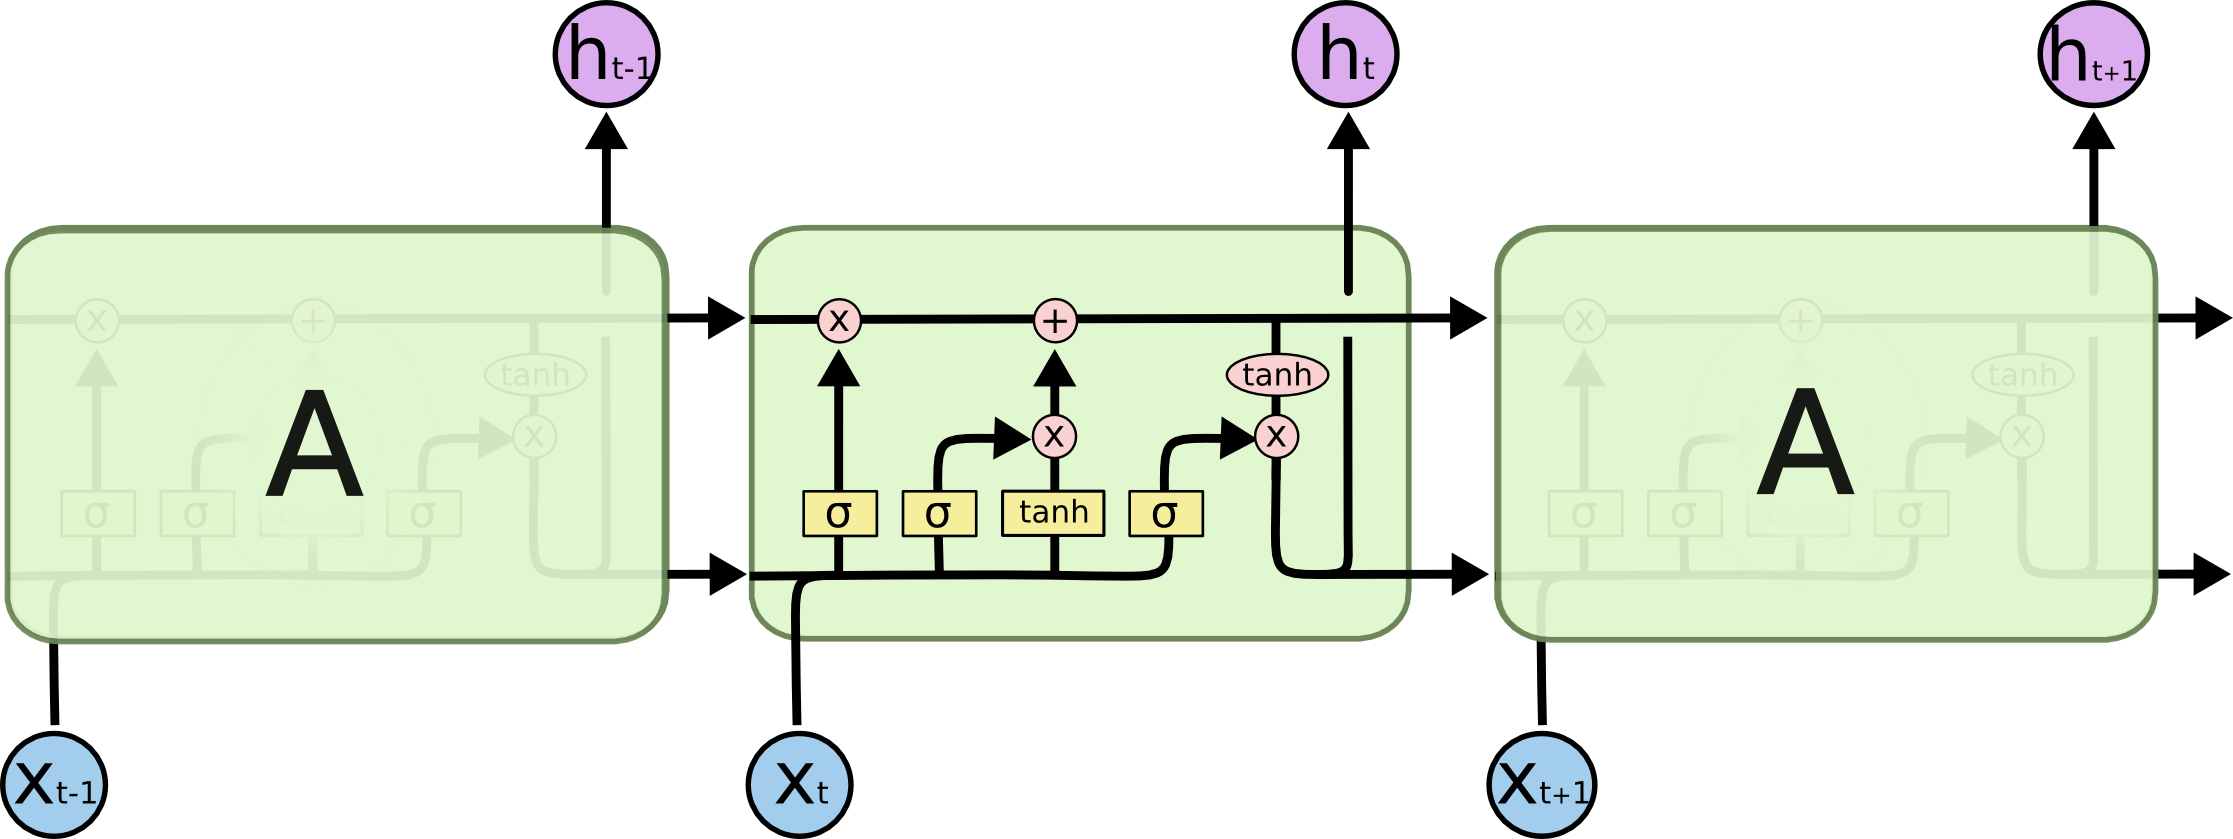
\includegraphics[width=0.4\textwidth]{LSTM-chain.png}
    \caption{The architecture of a LSTM.}
    \label{fig:lstm}
\end{figure}

Without entering into specific details, LSTM networks are explicitly crafted to capture and model long-term dependencies within sequences of information. The network incorporates loops, enabling the propagation and retention of information over time, essentially serving as a form of memory. In this specific context, a sequence refers to a subset of a weather time series with a length of $p$, denoted as $\{x_1, x_2, \ldots, x_p\}$, where $p < N$ represents the sequence length corresponding to the number of preceding weather samples used for prediction. At the end of the LSTM network, there is a linear layer that compresses the output into a single floating-point value, representing the ultimate temperature forecast. The entire architecture is trained via backpropagation, and the hyperparameters are detailed as follows:
\begin{itemize}
    \item \textbf{Sequence length}: the length of the sequence corresponding to the number of prior weather samples used for prediction.
    \item \textbf{LSTM hidden size}: the number of hidden units or neurons in each LSTM layer, determining the capacity of the model to capture complex patterns.
    \item \textbf{LSTM number of layers}: the number of stacked LSTM layers.
    \item \textbf{Optimizer learning rate}: the step size at which the optimizer adjusts the model weights during training.
    \item \textbf{Extra parameters list}: additional parameters beyond the outdoor temperature included as inputs, providing supplementary information for the model. Each element in the input sequence fed to the LSTM can be a vector of multiple features. Therefore, this hyperparameter aims to identify the weather parameters that enable the model to achieve optimal accuracy.
\end{itemize}

To employ genetic algorithms, various aspects must be defined, including the representation of the genotype for each individual, the selection mechanisms and the methods for individual mutation and crossover.


\subsubsection{Encoding of the Genotype}
In this specific context of hyperparameter tuning, the genotype is represented as an array containing the aforementioned hyperparameters, maintaining the same order. The order within the array is significant, as both the mutation and crossover operators are specifically tailored for this specific order.

\subsubsection{Crossover}
Crossover plays a pivotal role in emphasizing exploitation by combining optimal parts from different individuals. In this context, a uniform crossover operator is employed, selecting elements from the first and second individuals with equal probability.\\
% \subsubsection{Crossover}
% This method combines an arithmetic crossover operator for the initial four parameters and a uniform crossover operator for the last parameter. The arithmetic crossover computes the mean value of the two individuals for the first four parameters, while the uniform crossover randomly selects elements from the first and second individuals with equal probability for the last parameter.\\


\subsubsection{Mutation}
The first three parameters of the genotype (sequence length, LSTM hidden size, and LSTM number of layers) are integers, while the remaining ones are a float (the learning rate) and an array (the set of extra parameters). Considering the distinct nature of each gene in the genotype, a custom mutation operator has been implemented. It introduces an integer/float perturbation following a normal distribution to the integer/float genes, respectively, with a magnitude proportional to a predefined standard deviation provided by the user. For the last element in the genotype, the set of extra parameters, one element is probabilistically removed and added based on a certain probability.\\


\subsubsection{Selection} 
In the context of parent selection, tournament selection has been employed, wherein individuals are randomly sampled and compared against each other in tournaments of size $K$. The fittest individual from each tournament is then chosen as a parent for the genetic operations. Moreover, survivor selection follows an elitism strategy, aiming to preserve the best individuals from the previous generation. \\


\subsubsection{Algorithm} 
The genetic algorithm can be outlined as follows:

\begin{enumerate}
    \item Randomly sample an initial population of individuals.
    \item Evaluate the fitness of all individuals in the population.
    \item Select parents for reproduction through tournament selection(parent selection).
    \item With a probability $p_{c}$, choose two individuals from the parents' pool and return a single individual by applying the crossover operator. The new individual is then reintroduced into the parent pool.
    \item With a probability $p_{m}$, pick one individual from the parents' pool and subject it to mutation.
    \item Select individuals for the next generation by employing elitism as the survivor selection method.
    \item Repeat from step 2 until a termination condition is met, such as reaching a specified number of generations.
\end{enumerate}


\subsection{Genetic Programming}
The prior approach, which uses deep learning to address the time series weather temperature forecasting problem, lacks a crucial aspect: interpretability. This lack push the exploration of a second methodology centered on Genetic Programming, with the primary goal of establishing an interpretable model for the problem at hand.

In Genetic Programming, individuals are characterized by tree-based structures that represent a program or equation. The objective is to evolve a computer program or equation capable of solving the problem by directly deducing relationships within the data, without any prior assumptions about the model. However, a significant challenge encountered in Genetic Programming lies in the requirement for a large population of individuals. The dimensions of the evolved programs or equations can quickly increase, necessitating a substantial number of individuals within the population to adequately navigate and explore the search space.

In this study, the objective of Genetic Programming is to evolve an arithmetic expression that effectively models the intricate relationships among various weather parameters. This evolved tree-based structure representing an expression should have the capacity to predict the outdoor temperature for the subsequent hour, relying solely on prior observations.


The tree-based structure consist of nodes, where:
\begin{itemize}
    \item The leaves of the tree derive values from the \textbf{terminal set} $T$, encompassing constants and all variables relevant to the problem. In the problem examined in this study, the terminal set is defined as $\{x_t, x_{t-1}, \ldots, x_{t-p+1}, e\}$, where $p$ represents the number of preceding samples used for prediction, and $e$ is an ephemeral constant randomly initialized.
    \item The inner nodes represent functions that establish relationships among nodes in the terminal set. Each function has an arity, indicating the number of arguments it accepts. In this instance, the \textbf{function set} is denoted as $F$ and contains the four basic arithmetic operations and the trigonometric functions, $\sin$ and $\cos$. Due to the impracticality of a priori checking all potential inputs with Genetic Programming, the division operator has been redefined to prevent a zero division error.
\end{itemize}

Since the genotype is represented as a tree-based structure, standard mutation and crossover operations need to be tailored accordingly. In the case a one-point crossover is used, wherein a random crossover point is chosen in each individual, and the sub-trees rooted at the selected point are exchanged between the individuals. Regarding mutations, a customized mutation operator is employed, incorporating three mutation strategies randomly chosen with equal probability:

\begin{itemize}
    \item \textbf{Shrink}: a random node in the tree is selected, and the entire sub-tree is replaced with a single node.
    \item \textbf{Increase}: this strategy inserts a new branch at a random position in the mutated individual.
    \item \textbf{Ephemeral Mutation}: this mutation alters one of the ephemeral variables by applying a random mutation.
\end{itemize}

The rationale behind this mutation operator is to mitigate the bloat problem. This approach gives trees the flexibility to grow or shrink with an equal probability, thus preventing excessive growth.




\section{Experiments}

The experiments are carried out using weather data from the year 2022 obtained from my personal weather station in northern Italy\cite{dataset}. The station records various weather parameters, including outdoor temperature, humidity, atmospheric pressure, wind speed, and dewpoint, at two-second intervals. Due to the substantial size of the dataset, approximately $5.5$ GB, the data is resampled. Specifically, the temperature recordings are aggregated to an hourly frequency, guided by the assumption that temperature changes within a few minutes are not characterized by abrupt fluctuations. This process reduces the dataset to approximately $9000$ samples. 

The dataset is partitioned into three sets for training, validation, and testing purposes. During the hyperparameter tuning of the LSTM using Genetic Algorithms, the training set is employed for training the model through backpropagation by minimizing the error on the training set. The validation set is used to assess the model's generalization capabilities, and the accuracy metric based on the Mean Absolute Error is calculated on the validation set, serving as the fitness function for Genetic Algorithms. Finally, the test set is used to compare the three models.

For the method involving Genetic Programming, the size of the training set is reduced to the first $100$ samples due to the impracticality of using the entire training set given the number of individuals in the population, which would require excessive time. The validation set is employed, similar to the other method, to measure the model's ability to generalize and select the model that exhibits better generalization without overfitting the training data.


\subsection{Implementation}

The implementation of both approaches discussed in this paper is implemented in Python and is publicly available on GitHub \cite{github-repo}. Specifically:
\begin{itemize}
    \item The Genetic Algorithms employed for hyperparameter tuning was developed from scratch leveraging PyTorch\cite{pytorch} as the backend for the deep learning part. PyTorch provides advanced tools for both automatic gradient tracking and backpropagation, along with a simple interface for implementing LSTM models.
    \item For the Genetic Programming model, the DEAP\cite{deap} open-source library is utilized. It has been adapted to suit the specific requirements of this study. More precisely, the evolutionary algorithm governing genetic programming is modified to calculate the accuracy on the validation set at the conclusion of each generation. This change is crucial for evaluating the model's generalization capabilities.
\end{itemize}



\section{Results}

The performance of the proposed models has been assessed across various configurations to leverage their capabilities. The outcomes for each model are presented in the subsequent sections, categorized by model. The results for the baseline are reported in the concluding section dedicated to the comparison, as this model do not have specific configurations.

\subsection{LSTM Model}

This is the slowest algorithm, as the evaluation of each individual in the population involves training a LSTM model for a specified number of epochs—set to $15$ in this instance. The initial population consists of $20$ randomly initialized individuals, and the algorithm runs for $30$ generations. The tournament size $K$ is set to $3$ and the number of elites preserved at each generation is set to $2$. The crossover rate $p_c$ and mutation rate $p_m$ are respectively set to $p_c=0.3$ and $p_m=0.7$. The entire experiment takes several minutes, and the fitness progress over the generations is depicted in Figure \ref{fig:fitness-lstm}, where the plot illustrates the best model's fitness evaluated on the validation set at the end of each generation.

\begin{figure}[h]
\centering
    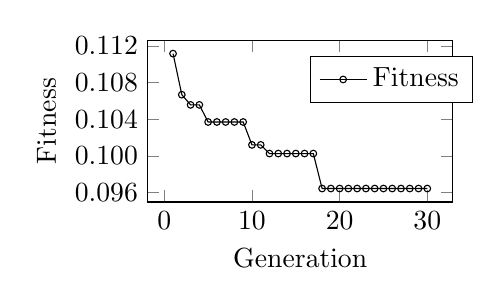
\begin{tikzpicture}
      \begin{axis}[
        xlabel={Generation},
        ylabel={Fitness},
        width=0.45\textwidth,
        height=0.3\textwidth,
        legend style={at={(0.8, 0.9)},anchor=north},
        mark size=1.2,
        y tick label style={/pgf/number format/.cd,fixed,fixed zerofill=true,precision=3},
        ytick={0.096,0.100,...,0.12},
      ]
      
      \addplot[mark=o] coordinates {
        (1, 0.111149)
        (2, 0.106667)
        (3, 0.105555)
        (4, 0.105555)
        (5, 0.103689)
        (6, 0.103689)
        (7, 0.103689)
        (8, 0.103689)
        (9, 0.103689)
        (10, 0.101192)
        (11, 0.101192)
        (12, 0.100245)
        (13, 0.100245)
        (14, 0.100245)
        (15, 0.100245)
        (16, 0.100245)
        (17, 0.100245)
        (18, 0.096430)
        (19, 0.096430)
        (20, 0.096430)
        (21, 0.096430)
        (22, 0.096430)
        (23, 0.096430)
        (24, 0.096430)
        (25, 0.096430)
        (26, 0.096430)
        (27, 0.096430)
        (28, 0.096430)
        (29, 0.096430)
        (30, 0.096430)
      };
      
      \legend{Fitness}
      \end{axis}
    
    \end{tikzpicture}
\caption{Change in fitness over generations.} 
\label{fig:fitness-lstm}
\end{figure}

The best individual reported by Genetic Algorithms has a fitness of $0.0984$ on the validation set, and the optimal configuration found is \verb|[61, 33, 1, 0.0044261263, []]|. Interestingly, the model did not incorporate any additional weather parameters beyond the outdoor temperature, indicating that these omitted parameters may not have played a crucial role in the forecasting process.

\subsection{Genetic Programming}

In this particular case, the problem space is large, necessitating a substantial population. Specifically, the population size is configured with $500$ individuals, and the tournament size $K$ is set to $5$. A range of values for the crossover rate $p_c$ and mutation rate $p_m$ has been explored, yielding notably diverse outcomes. The optimal tree is derived with $p_c=0.8$ and $p_m=0.1$, executing over a span of $20$ generations. The visual representation of the evolved tree is provided in Figure \ref{fig:gp-tree}, where $\{x_0, x_1, x_2, x_3\}$ denotes the past $p=4$, with $x_3$ being the latest one, and $e_0=0.17488$ and $e_1=0.97058$ represent ephemeral variables. The fitness progress over the generations is depicted in Figure \ref{fig:gp-evolution}, where the plot illustrates the best model’s fitness evaluated
on the training set at the end of each generation as well as the average size of the evolved trees.

An interesting observation arises from the evolved tree structure: only the initial and final temperature observations are employed to forecast the temperature of the next hour while the intermediate measurements of the temperature are disregarded in this predictive process. This distinctive characteristic adds nuance to the understanding of how the Genetic Programming model interprets and utilizes past observations and ephemeral variables in forecasting.

\begin{figure}[h]
\centering
    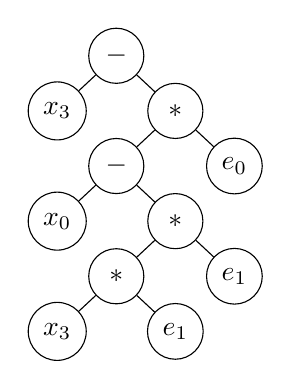
\begin{tikzpicture}[
      every node/.style={circle, draw, minimum size=7mm},
      level distance=7mm,
      sibling distance=15mm,
    ]
    \node {$-$}
      child {node {$x_3$}}
      child {node {$*$}
        child {node {$-$}
          child {node {$x_0$}}
          child {node {$*$}
            child {node {$*$}
              child {node {$x_3$}}
              child {node {$e_1$}}
            }
            child {node {$e_1$}}
          }
        }
        child {node {$e_0$}}
      };
    \end{tikzpicture}    
\caption{Evolved tree generated by Genetic Programming.} 
\label{fig:gp-tree}
\end{figure}


\begin{figure}
    \centering
    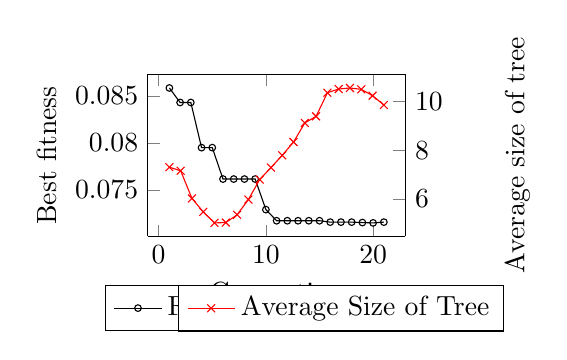
\begin{tikzpicture}
    
      \begin{axis}[
        xlabel={Generation},
        ylabel={Best fitness},
        axis y line*=left,
        legend style={at={(0.15,-0.3)}, anchor=north, legend columns=-1},
        yticklabel style={
            /pgf/number format/fixed,
            /pgf/number format/precision=5
        },
        width=0.4\textwidth,
        height=0.3\textwidth,
        scaled y ticks=false,
        mark size=1.2,
      ]
      
      \addplot[mark=o, black] coordinates {
          (1, 0.08584692178901428)
          (2, 0.08430659472942352)
          (3, 0.08430659472942352)
          (4, 0.07950782254907311)
          (5, 0.07950782254907311)
          (6, 0.07617175246263186)
          (7, 0.07617175246263186)
          (8, 0.07617175246263186)
          (9, 0.07617175246263186)
          (10, 0.07292518568784243)
          (11, 0.07174215158304403)
          (12, 0.07174215158304403)
          (13, 0.07174215158304403)
          (14, 0.07174215158304403)
          (15, 0.07174215158304403)
          (16, 0.07159554874702596)
          (17, 0.07159554874702596)
          (18, 0.07159554874702596)
          (19, 0.07154947389260462)
          (20, 0.07151369182701221)
          (21, 0.07159554874702596)
      };
      
      \legend{Fitness}
      
      \end{axis}
      
      \begin{axis}[
        axis x line=none,
        axis y line*=right,
        ylabel={Average size of tree},
        y label style={at={(1.35,0.5)}},
        legend style={at={(0.75,-0.3)}, anchor=north, legend columns=-1},
        width=0.4\textwidth,
        height=0.3\textwidth,
      ]
      
      \addplot[mark=x, red] coordinates {
          (1, 7.308)
          (2, 7.16)
          (3, 6.024)
          (4, 5.472)
          (5, 5.018)
          (6, 5.032)
          (7, 5.35)
          (8, 5.978)
          (9, 6.8)
          (10, 7.292)
          (11, 7.796)
          (12, 8.342)
          (13, 9.128)
          (14, 9.398)
          (15, 10.37)
          (16, 10.52)
          (17, 10.564)
          (18, 10.508)
          (19, 10.248)
          (20, 9.864)
      };
      
      \legend{Average Size of Tree}
      
      \end{axis}
    \end{tikzpicture}

\caption{Fitness trend and average tree size over generations.} 
\label{fig:gp-evolution}
\end{figure}

\subsection{Comparison}

All the three models were tested on the test split of the dataset, containing the data of the last half of the year, obtaining the results reported in Table \ref{results}. The results detailed in Table \ref{results}, distinctly demonstrate the LSTM-based model's superior performance in terms of Mean Absolute Error. However, in terms of complexity, Genetic Programming produced an interpretable model for the given problem, characterized by basic arithmetic operations. In contrast, the LSTM model involved a more intricate structure with a total of $3501$ parameters.

\begin{table}[htbp]
  \centering
  \begin{tabular}{lccc}
    \toprule
     & \textbf{Baseline} & \textbf{LSTM} & \textbf{GP} \\
    \midrule
    \textbf{MAE} & 0.1126 & 0.08005 & 0.0929 \\
    \bottomrule
  \end{tabular}
  \caption{MAE values for different models}
  \label{results}
\end{table}

\section{Conclusion}
In summary, the obtained results reveal that Genetic Programming produced satisfactory outcomes, albeit with a slightly inferior performance compared to LSTM in terms of MAE. Despite LSTM's superior performance, the evolved mathematical expression might be favored for its simplicity and interpretability, particularly in scenarios where computational cost and efficiency are fundamental. It is crucial to note that this study exclusively utilized outdoor temperature, neglecting other parameters. Acknowledging the potential existence of intrinsic relationships among various weather parameters, future research endeavors should encompass a more comprehensive exploration of the search space to unearth improved solutions by exploiting the interdependencies within the complete set of weather data.







% if have a single appendix:
%\appendix[Proof of the Zonklar Equations]
% or
%\appendix  % for no appendix heading
% do not use \section anymore after \appendix, only \section*
% is possibly needed

% use appendices with more than one appendix
% then use \section to start each appendix
% you must declare a \section before using any
% \subsection or using \label (\appendices by itself
% starts a section numbered zero.)
%





% trigger a \newpage just before the given reference
% number - used to balance the columns on the last page
% adjust value as needed - may need to be readjusted if
% the document is modified later
%\IEEEtriggeratref{8}
% The "triggered" command can be changed if desired:
%\IEEEtriggercmd{\enlargethispage{-5in}}

% references section

% can use a bibliography generated by BibTeX as a .bbl file
% BibTeX documentation can be easily obtained at:
% http://mirror.ctan.org/biblio/bibtex/contrib/doc/
% The IEEEtran BibTeX style support page is at:
% http://www.michaelshell.org/tex/ieeetran/bibtex/
%\bibliographystyle{IEEEtran}
% argument is your BibTeX string definitions and bibliography database(s)
%\bibliography{IEEEabrv,../bib/paper}
%
% <OR> manually copy in the resultant .bbl file
% set second argument of \begin to the number of references
% (used to reserve space for the reference number labels box)
\bibliographystyle{./bibtex/bib/IEEEtran.bst}
\bibliography{bibtex/bib/references} 

\onecolumn
\appendices

\section{Qualitative results}

\begin{figure}[h]
    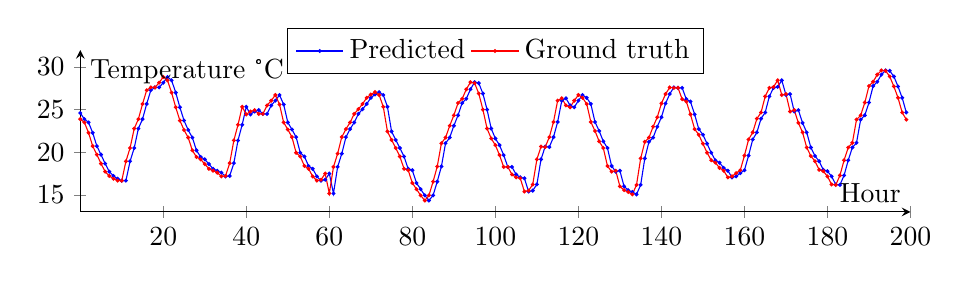
\begin{tikzpicture}
      \pgfplotsset{every axis legend/.append style={
        at={(0.5,0.85)},
        anchor=south},
        legend columns=-1}
      \begin{axis}[
            xlabel={Hour},
            ylabel={Temperature °C},
            width=\textwidth,
            height=0.3\textwidth,
            mark size=0.5,
            xmin=0, xmax=200,
            ymin=13, ymax=32,
            axis lines=middle
        ]
    
        \addplot[blue, mark=*] coordinates {
            (0, 24.611111)
            (1, 23.888890)
            (2, 23.499999)
            (3, 22.277778)
            (4, 20.722222)
            (5, 19.722222)
            (6, 18.666667)
            (7, 17.722222)
            (8, 17.222222)
            (9, 16.888889)
            (10, 16.666667)
            (11, 16.666667)
            (12, 18.944444)
            (13, 20.500000)
            (14, 22.777778)
            (15, 23.888890)
            (16, 25.666667)
            (17, 27.277777)
            (18, 27.611112)
            (19, 27.611112)
            (20, 28.166667)
            (21, 28.833334)
            (22, 28.444444)
            (23, 27.000000)
            (24, 25.277777)
            (25, 23.722222)
            (26, 22.611111)
            (27, 21.722222)
            (28, 20.222222)
            (29, 19.444444)
            (30, 19.166667)
            (31, 18.611111)
            (32, 18.055556)
            (33, 17.833333)
            (34, 17.611111)
            (35, 17.166667)
            (36, 17.222222)
            (37, 18.722222)
            (38, 21.388889)
            (39, 23.222222)
            (40, 25.333333)
            (41, 24.444445)
            (42, 24.777778)
            (43, 24.944444)
            (44, 24.499999)
            (45, 24.499999)
            (46, 25.499999)
            (47, 26.055556)
            (48, 26.722222)
            (49, 25.611111)
            (50, 23.499999)
            (51, 22.666666)
            (52, 21.777777)
            (53, 19.944445)
            (54, 19.500000)
            (55, 18.388889)
            (56, 18.055556)
            (57, 17.166667)
            (58, 16.666667)
            (59, 16.777778)
            (60, 17.500000)
            (61, 15.166667)
            (62, 18.277778)
            (63, 19.833333)
            (64, 21.777777)
            (65, 22.722222)
            (66, 23.499999)
            (67, 24.499999)
            (68, 25.055556)
            (69, 25.666667)
            (70, 26.388889)
            (71, 26.777778)
            (72, 27.055555)
            (73, 26.722222)
            (74, 25.333333)
            (75, 22.444445)
            (76, 21.444445)
            (77, 20.500000)
            (78, 19.500000)
            (79, 18.055556)
            (80, 17.888889)
            (81, 16.388889)
            (82, 15.666667)
            (83, 14.944445)
            (84, 14.333333)
            (85, 14.944445)
            (86, 16.555555)
            (87, 18.333333)
            (88, 21.055556)
            (89, 21.722222)
            (90, 23.111110)
            (91, 24.333333)
            (92, 25.777778)
            (93, 26.277777)
            (94, 27.388889)
            (95, 28.222223)
            (96, 28.111111)
            (97, 26.888888)
            (98, 25.000000)
            (99, 22.777778)
            (100, 21.611111)
            (101, 20.833333)
            (102, 19.666667)
            (103, 18.277778)
            (104, 18.277778)
            (105, 17.388889)
            (106, 17.055555)
            (107, 16.944444)
            (108, 15.388889)
            (109, 15.500000)
            (110, 16.222223)
            (111, 19.166667)
            (112, 20.666667)
            (113, 20.611111)
            (114, 21.777777)
            (115, 23.555555)
            (116, 26.055556)
            (117, 26.333333)
            (118, 25.499999)
            (119, 25.277777)
            (120, 26.055556)
            (121, 26.722222)
            (122, 26.388889)
            (123, 25.666667)
            (124, 23.555555)
            (125, 22.500000)
            (126, 21.277777)
            (127, 20.500000)
            (128, 18.388889)
            (129, 17.722222)
            (130, 17.833333)
            (131, 16.000000)
            (132, 15.555555)
            (133, 15.333333)
            (134, 15.055556)
            (135, 16.166667)
            (136, 19.277778)
            (137, 21.222222)
            (138, 21.722222)
            (139, 23.000000)
            (140, 24.111110)
            (141, 25.722222)
            (142, 26.833334)
            (143, 27.611112)
            (144, 27.555556)
            (145, 27.555556)
            (146, 26.222223)
            (147, 25.944444)
            (148, 24.444445)
            (149, 22.722222)
            (150, 22.055556)
            (151, 21.000000)
            (152, 19.944445)
            (153, 19.055556)
            (154, 18.777778)
            (155, 18.166667)
            (156, 17.833333)
            (157, 17.055555)
            (158, 17.166667)
            (159, 17.555556)
            (160, 17.888889)
            (161, 19.611111)
            (162, 21.500000)
            (163, 22.333334)
            (164, 23.944444)
            (165, 24.666667)
            (166, 26.555556)
            (167, 27.555556)
            (168, 27.666666)
            (169, 28.444444)
            (170, 26.722222)
            (171, 26.833334)
            (172, 24.777778)
            (173, 24.944444)
            (174, 23.444445)
            (175, 22.333334)
            (176, 20.555556)
            (177, 19.555556)
            (178, 18.944444)
            (179, 17.944444)
            (180, 17.777778)
            (181, 17.166667)
            (182, 16.222223)
            (183, 16.166667)
            (184, 17.277778)
            (185, 19.055556)
            (186, 20.555556)
            (187, 21.111111)
            (188, 23.833334)
            (189, 24.333333)
            (190, 25.833334)
            (191, 27.777778)
            (192, 28.277777)
            (193, 29.111111)
            (194, 29.611112)
            (195, 29.555556)
            (196, 28.888888)
            (197, 27.722222)
            (198, 26.388889)
            (199, 24.666667)
            
        };
        \addlegendentry{Predicted}
    
        \addplot[red, mark=*] coordinates {
            (0, 23.888890)
            (1, 23.499999)
            (2, 22.277778)
            (3, 20.722222)
            (4, 19.722222)
            (5, 18.666667)
            (6, 17.722222)
            (7, 17.222222)
            (8, 16.888889)
            (9, 16.666667)
            (10, 16.666667)
            (11, 18.944444)
            (12, 20.500000)
            (13, 22.777778)
            (14, 23.888890)
            (15, 25.666667)
            (16, 27.277777)
            (17, 27.611112)
            (18, 27.611112)
            (19, 28.166667)
            (20, 28.833334)
            (21, 28.444444)
            (22, 27.000000)
            (23, 25.277777)
            (24, 23.722222)
            (25, 22.611111)
            (26, 21.722222)
            (27, 20.222222)
            (28, 19.444444)
            (29, 19.166667)
            (30, 18.611111)
            (31, 18.055556)
            (32, 17.833333)
            (33, 17.611111)
            (34, 17.166667)
            (35, 17.222222)
            (36, 18.722222)
            (37, 21.388889)
            (38, 23.222222)
            (39, 25.333333)
            (40, 24.444445)
            (41, 24.777778)
            (42, 24.944444)
            (43, 24.499999)
            (44, 24.499999)
            (45, 25.499999)
            (46, 26.055556)
            (47, 26.722222)
            (48, 25.611111)
            (49, 23.499999)
            (50, 22.666666)
            (51, 21.777777)
            (52, 19.944445)
            (53, 19.500000)
            (54, 18.388889)
            (55, 18.055556)
            (56, 17.166667)
            (57, 16.666667)
            (58, 16.777778)
            (59, 17.500000)
            (60, 15.166667)
            (61, 18.277778)
            (62, 19.833333)
            (63, 21.777777)
            (64, 22.722222)
            (65, 23.499999)
            (66, 24.499999)
            (67, 25.055556)
            (68, 25.666667)
            (69, 26.388889)
            (70, 26.777778)
            (71, 27.055555)
            (72, 26.722222)
            (73, 25.333333)
            (74, 22.444445)
            (75, 21.444445)
            (76, 20.500000)
            (77, 19.500000)
            (78, 18.055556)
            (79, 17.888889)
            (80, 16.388889)
            (81, 15.666667)
            (82, 14.944445)
            (83, 14.333333)
            (84, 14.944445)
            (85, 16.555555)
            (86, 18.333333)
            (87, 21.055556)
            (88, 21.722222)
            (89, 23.111110)
            (90, 24.333333)
            (91, 25.777778)
            (92, 26.277777)
            (93, 27.388889)
            (94, 28.222223)
            (95, 28.111111)
            (96, 26.888888)
            (97, 25.000000)
            (98, 22.777778)
            (99, 21.611111)
            (100, 20.833333)
            (101, 19.666667)
            (102, 18.277778)
            (103, 18.277778)
            (104, 17.388889)
            (105, 17.055555)
            (106, 16.944444)
            (107, 15.388889)
            (108, 15.500000)
            (109, 16.222223)
            (110, 19.166667)
            (111, 20.666667)
            (112, 20.611111)
            (113, 21.777777)
            (114, 23.555555)
            (115, 26.055556)
            (116, 26.333333)
            (117, 25.499999)
            (118, 25.277777)
            (119, 26.055556)
            (120, 26.722222)
            (121, 26.388889)
            (122, 25.666667)
            (123, 23.555555)
            (124, 22.500000)
            (125, 21.277777)
            (126, 20.500000)
            (127, 18.388889)
            (128, 17.722222)
            (129, 17.833333)
            (130, 16.000000)
            (131, 15.555555)
            (132, 15.333333)
            (133, 15.055556)
            (134, 16.166667)
            (135, 19.277778)
            (136, 21.222222)
            (137, 21.722222)
            (138, 23.000000)
            (139, 24.111110)
            (140, 25.722222)
            (141, 26.833334)
            (142, 27.611112)
            (143, 27.555556)
            (144, 27.555556)
            (145, 26.222223)
            (146, 25.944444)
            (147, 24.444445)
            (148, 22.722222)
            (149, 22.055556)
            (150, 21.000000)
            (151, 19.944445)
            (152, 19.055556)
            (153, 18.777778)
            (154, 18.166667)
            (155, 17.833333)
            (156, 17.055555)
            (157, 17.166667)
            (158, 17.555556)
            (159, 17.888889)
            (160, 19.611111)
            (161, 21.500000)
            (162, 22.333334)
            (163, 23.944444)
            (164, 24.666667)
            (165, 26.555556)
            (166, 27.555556)
            (167, 27.666666)
            (168, 28.444444)
            (169, 26.722222)
            (170, 26.833334)
            (171, 24.777778)
            (172, 24.944444)
            (173, 23.444445)
            (174, 22.333334)
            (175, 20.555556)
            (176, 19.555556)
            (177, 18.944444)
            (178, 17.944444)
            (179, 17.777778)
            (180, 17.166667)
            (181, 16.222223)
            (182, 16.166667)
            (183, 17.277778)
            (184, 19.055556)
            (185, 20.555556)
            (186, 21.111111)
            (187, 23.833334)
            (188, 24.333333)
            (189, 25.833334)
            (190, 27.777778)
            (191, 28.277777)
            (192, 29.111111)
            (193, 29.611112)
            (194, 29.555556)
            (195, 28.888888)
            (196, 27.722222)
            (197, 26.388889)
            (198, 24.666667)
            (199, 23.833334)
            
        };
        \addlegendentry{Ground truth}
    
      \end{axis}
    \end{tikzpicture}

    \caption{\textbf{Baseline} model evaluated on the first $200$ samples of the test set.} 
    \label{fig:baseline-pred}
\end{figure}


\begin{figure}[h]
    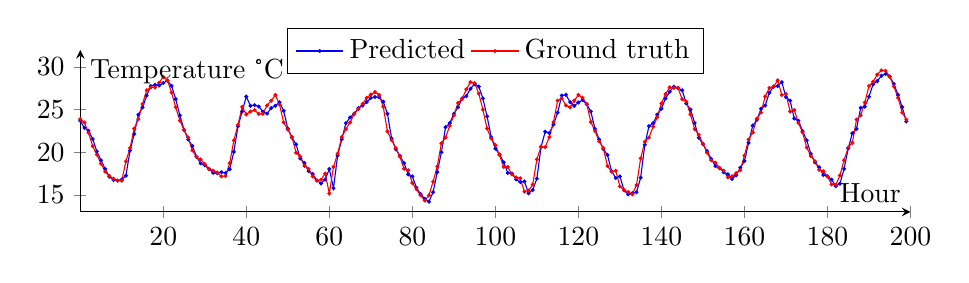
\begin{tikzpicture}
      \pgfplotsset{every axis legend/.append style={
        at={(0.5,0.85)},
        anchor=south},
        legend columns=-1}
      \begin{axis}[
            xlabel={Hour},
            ylabel={Temperature °C},
            width=\textwidth,
            height=0.3\textwidth,
            mark size=0.5,
            xmin=0, xmax=200,
            ymin=13, ymax=32,
            axis lines=middle
        ]
    
        \addplot[blue, mark=*] coordinates {
            (0, 23.691763)
            (1, 22.862778)
            (2, 22.523911)
            (3, 21.558778)
            (4, 20.096254)
            (5, 19.053852)
            (6, 18.041753)
            (7, 17.130724)
            (8, 16.741980)
            (9, 16.672277)
            (10, 16.809810)
            (11, 17.246879)
            (12, 20.211144)
            (13, 22.143607)
            (14, 24.410945)
            (15, 25.260653)
            (16, 26.643325)
            (17, 27.775609)
            (18, 27.917720)
            (19, 27.826467)
            (20, 28.124793)
            (21, 28.406792)
            (22, 27.798839)
            (23, 26.240840)
            (24, 24.332468)
            (25, 22.629299)
            (26, 21.498349)
            (27, 20.743385)
            (28, 19.482186)
            (29, 18.700396)
            (30, 18.471138)
            (31, 18.040811)
            (32, 17.578798)
            (33, 17.552619)
            (34, 17.659861)
            (35, 17.561262)
            (36, 18.016958)
            (37, 20.053898)
            (38, 23.047140)
            (39, 24.773809)
            (40, 26.539597)
            (41, 25.449789)
            (42, 25.530456)
            (43, 25.371501)
            (44, 24.756740)
            (45, 24.540846)
            (46, 25.186711)
            (47, 25.452969)
            (48, 25.857408)
            (49, 24.866726)
            (50, 22.767091)
            (51, 21.722934)
            (52, 20.923682)
            (53, 19.284737)
            (54, 18.747878)
            (55, 17.786734)
            (56, 17.447354)
            (57, 16.699055)
            (58, 16.332749)
            (59, 16.787907)
            (60, 18.036692)
            (61, 15.784053)
            (62, 19.603452)
            (63, 21.537423)
            (64, 23.416571)
            (65, 24.084918)
            (66, 24.542675)
            (67, 25.189906)
            (68, 25.478371)
            (69, 25.889326)
            (70, 26.371463)
            (71, 26.487942)
            (72, 26.452312)
            (73, 25.934167)
            (74, 24.515723)
            (75, 21.640021)
            (76, 20.368685)
            (77, 19.554062)
            (78, 18.728692)
            (79, 17.402043)
            (80, 17.164898)
            (81, 15.825663)
            (82, 15.071897)
            (83, 14.545646)
            (84, 14.200094)
            (85, 15.312255)
            (86, 17.668092)
            (87, 20.007371)
            (88, 22.943789)
            (89, 23.410926)
            (90, 24.504058)
            (91, 25.283084)
            (92, 26.322700)
            (93, 26.584100)
            (94, 27.453596)
            (95, 28.012771)
            (96, 27.705753)
            (97, 26.326084)
            (98, 24.210680)
            (99, 21.769771)
            (100, 20.418182)
            (101, 19.736783)
            (102, 18.826861)
            (103, 17.572714)
            (104, 17.513688)
            (105, 16.817330)
            (106, 16.497011)
            (107, 16.572987)
            (108, 15.187021)
            (109, 15.569172)
            (110, 16.912768)
            (111, 20.612612)
            (112, 22.413942)
            (113, 22.262276)
            (114, 23.246764)
            (115, 24.647967)
            (116, 26.659685)
            (117, 26.736906)
            (118, 25.879874)
            (119, 25.445619)
            (120, 25.837631)
            (121, 26.129630)
            (122, 25.632678)
            (123, 24.785699)
            (124, 22.729199)
            (125, 21.501576)
            (126, 20.384654)
            (127, 19.689520)
            (128, 17.784897)
            (129, 16.972141)
            (130, 17.175763)
            (131, 15.525070)
            (132, 15.066025)
            (133, 15.197876)
            (134, 15.308960)
            (135, 17.016104)
            (136, 20.894452)
            (137, 23.058306)
            (138, 23.413904)
            (139, 24.416591)
            (140, 25.112933)
            (141, 26.310551)
            (142, 27.105326)
            (143, 27.704032)
            (144, 27.544078)
            (145, 27.269435)
            (146, 25.727236)
            (147, 25.004047)
            (148, 23.452961)
            (149, 21.696185)
            (150, 20.959733)
            (151, 20.130174)
            (152, 19.211406)
            (153, 18.378508)
            (154, 18.121803)
            (155, 17.638930)
            (156, 17.418906)
            (157, 16.855802)
            (158, 17.296182)
            (159, 18.190033)
            (160, 18.962042)
            (161, 21.112635)
            (162, 23.127108)
            (163, 23.794355)
            (164, 25.110506)
            (165, 25.480707)
            (166, 26.980554)
            (167, 27.710958)
            (168, 27.759200)
            (169, 28.230789)
            (170, 26.479568)
            (171, 26.058525)
            (172, 23.960543)
            (173, 23.709305)
            (174, 22.476335)
            (175, 21.411084)
            (176, 19.811480)
            (177, 18.792265)
            (178, 18.238742)
            (179, 17.335413)
            (180, 17.192617)
            (181, 16.790325)
            (182, 16.026285)
            (183, 16.308475)
            (184, 18.047785)
            (185, 20.449898)
            (186, 22.234389)
            (187, 22.740189)
            (188, 25.215119)
            (189, 25.349527)
            (190, 26.512145)
            (191, 27.973981)
            (192, 28.347213)
            (193, 28.981996)
            (194, 29.198720)
            (195, 28.881925)
            (196, 28.023835)
            (197, 26.732975)
            (198, 25.301503)
            (199, 23.611199)
        };
        \addlegendentry{Predicted}
    
        \addplot[red, mark=*] coordinates {
            (0, 23.888890)
            (1, 23.499999)
            (2, 22.277778)
            (3, 20.722222)
            (4, 19.722222)
            (5, 18.666667)
            (6, 17.722222)
            (7, 17.222222)
            (8, 16.888889)
            (9, 16.666667)
            (10, 16.666667)
            (11, 18.944444)
            (12, 20.500000)
            (13, 22.777778)
            (14, 23.888890)
            (15, 25.666667)
            (16, 27.277777)
            (17, 27.611112)
            (18, 27.611112)
            (19, 28.166667)
            (20, 28.833334)
            (21, 28.444444)
            (22, 27.000000)
            (23, 25.277777)
            (24, 23.722222)
            (25, 22.611111)
            (26, 21.722222)
            (27, 20.222222)
            (28, 19.444444)
            (29, 19.166667)
            (30, 18.611111)
            (31, 18.055556)
            (32, 17.833333)
            (33, 17.611111)
            (34, 17.166667)
            (35, 17.222222)
            (36, 18.722222)
            (37, 21.388889)
            (38, 23.222222)
            (39, 25.333333)
            (40, 24.444445)
            (41, 24.777778)
            (42, 24.944444)
            (43, 24.499999)
            (44, 24.499999)
            (45, 25.499999)
            (46, 26.055556)
            (47, 26.722222)
            (48, 25.611111)
            (49, 23.499999)
            (50, 22.666666)
            (51, 21.777777)
            (52, 19.944445)
            (53, 19.500000)
            (54, 18.388889)
            (55, 18.055556)
            (56, 17.166667)
            (57, 16.666667)
            (58, 16.777778)
            (59, 17.500000)
            (60, 15.166667)
            (61, 18.277778)
            (62, 19.833333)
            (63, 21.777777)
            (64, 22.722222)
            (65, 23.499999)
            (66, 24.499999)
            (67, 25.055556)
            (68, 25.666667)
            (69, 26.388889)
            (70, 26.777778)
            (71, 27.055555)
            (72, 26.722222)
            (73, 25.333333)
            (74, 22.444445)
            (75, 21.444445)
            (76, 20.500000)
            (77, 19.500000)
            (78, 18.055556)
            (79, 17.888889)
            (80, 16.388889)
            (81, 15.666667)
            (82, 14.944445)
            (83, 14.333333)
            (84, 14.944445)
            (85, 16.555555)
            (86, 18.333333)
            (87, 21.055556)
            (88, 21.722222)
            (89, 23.111110)
            (90, 24.333333)
            (91, 25.777778)
            (92, 26.277777)
            (93, 27.388889)
            (94, 28.222223)
            (95, 28.111111)
            (96, 26.888888)
            (97, 25.000000)
            (98, 22.777778)
            (99, 21.611111)
            (100, 20.833333)
            (101, 19.666667)
            (102, 18.277778)
            (103, 18.277778)
            (104, 17.388889)
            (105, 17.055555)
            (106, 16.944444)
            (107, 15.388889)
            (108, 15.500000)
            (109, 16.222223)
            (110, 19.166667)
            (111, 20.666667)
            (112, 20.611111)
            (113, 21.777777)
            (114, 23.555555)
            (115, 26.055556)
            (116, 26.333333)
            (117, 25.499999)
            (118, 25.277777)
            (119, 26.055556)
            (120, 26.722222)
            (121, 26.388889)
            (122, 25.666667)
            (123, 23.555555)
            (124, 22.500000)
            (125, 21.277777)
            (126, 20.500000)
            (127, 18.388889)
            (128, 17.722222)
            (129, 17.833333)
            (130, 16.000000)
            (131, 15.555555)
            (132, 15.333333)
            (133, 15.055556)
            (134, 16.166667)
            (135, 19.277778)
            (136, 21.222222)
            (137, 21.722222)
            (138, 23.000000)
            (139, 24.111110)
            (140, 25.722222)
            (141, 26.833334)
            (142, 27.611112)
            (143, 27.555556)
            (144, 27.555556)
            (145, 26.222223)
            (146, 25.944444)
            (147, 24.444445)
            (148, 22.722222)
            (149, 22.055556)
            (150, 21.000000)
            (151, 19.944445)
            (152, 19.055556)
            (153, 18.777778)
            (154, 18.166667)
            (155, 17.833333)
            (156, 17.055555)
            (157, 17.166667)
            (158, 17.555556)
            (159, 17.888889)
            (160, 19.611111)
            (161, 21.500000)
            (162, 22.333334)
            (163, 23.944444)
            (164, 24.666667)
            (165, 26.555556)
            (166, 27.555556)
            (167, 27.666666)
            (168, 28.444444)
            (169, 26.722222)
            (170, 26.833334)
            (171, 24.777778)
            (172, 24.944444)
            (173, 23.444445)
            (174, 22.333334)
            (175, 20.555556)
            (176, 19.555556)
            (177, 18.944444)
            (178, 17.944444)
            (179, 17.777778)
            (180, 17.166667)
            (181, 16.222223)
            (182, 16.166667)
            (183, 17.277778)
            (184, 19.055556)
            (185, 20.555556)
            (186, 21.111111)
            (187, 23.833334)
            (188, 24.333333)
            (189, 25.833334)
            (190, 27.777778)
            (191, 28.277777)
            (192, 29.111111)
            (193, 29.611112)
            (194, 29.555556)
            (195, 28.888888)
            (196, 27.722222)
            (197, 26.388889)
            (198, 24.666667)
            (199, 23.833334)         
        };
        \addlegendentry{Ground truth}
    
      \end{axis}
    \end{tikzpicture}

    \caption{\textbf{LSTM} model evaluated on the first $200$ samples of the test set.} 
    \label{fig:lstm-pred}
\end{figure}



\begin{figure}[h]
    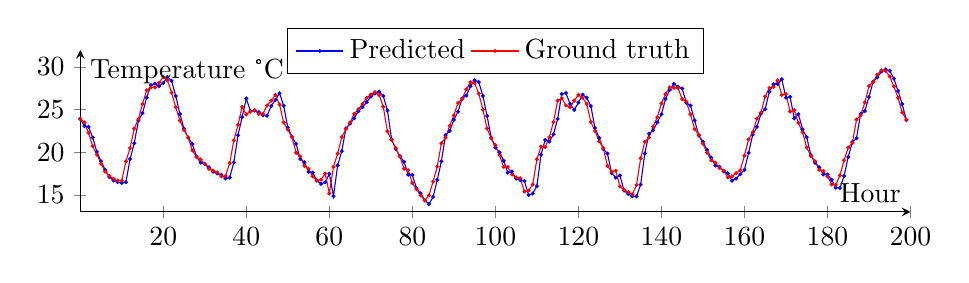
\begin{tikzpicture}
      \pgfplotsset{every axis legend/.append style={
        at={(0.5,0.85)},
        anchor=south},
        legend columns=-1}
      \begin{axis}[
            xlabel={Hour},
            ylabel={Temperature °C},
            width=\textwidth,
            height=0.3\textwidth,
            mark size=0.5,
            xmin=0, xmax=200,
            ymin=13, ymax=32,
            axis lines=middle,
        ]
    
        \addplot[blue, mark=*] coordinates {
            (0, 23.935157)
            (1, 23.074520)
            (2, 22.981043)
            (3, 21.732347)
            (4, 20.046823)
            (5, 18.950087)
            (6, 17.934378)
            (7, 17.106379)
            (8, 16.698889)
            (9, 16.495239)
            (10, 16.401574)
            (11, 16.489015)
            (12, 19.200344)
            (13, 21.051036)
            (14, 23.704071)
            (15, 24.599890)
            (16, 26.398511)
            (17, 27.876701)
            (18, 28.070636)
            (19, 27.759733)
            (20, 28.125058)
            (21, 28.843262)
            (22, 28.390303)
            (23, 26.610735)
            (24, 24.488192)
            (25, 22.744374)
            (26, 21.702820)
            (27, 20.968677)
            (28, 19.493597)
            (29, 18.781997)
            (30, 18.613909)
            (31, 18.229151)
            (32, 17.718090)
            (33, 17.507836)
            (34, 17.346160)
            (35, 16.925653)
            (36, 17.029224)
            (37, 18.815207)
            (38, 21.998925)
            (39, 24.124579)
            (40, 26.321164)
            (41, 24.819479)
            (42, 24.887108)
            (43, 24.712035)
            (44, 24.349820)
            (45, 24.291526)
            (46, 25.427126)
            (47, 26.151935)
            (48, 26.928432)
            (49, 25.459386)
            (50, 22.903317)
            (51, 21.816106)
            (52, 20.975090)
            (53, 19.208919)
            (54, 18.836990)
            (55, 17.698279)
            (56, 17.630649)
            (57, 16.673044)
            (58, 16.284985)
            (59, 16.472696)
            (60, 17.469354)
            (61, 14.839052)
            (62, 18.443278)
            (63, 20.128802)
            (64, 22.801648)
            (65, 23.357607)
            (66, 23.991479)
            (67, 24.816176)
            (68, 25.298091)
            (69, 25.873861)
            (70, 26.540184)
            (71, 26.895983)
            (72, 27.112650)
            (73, 26.598097)
            (74, 24.912383)
            (75, 21.498980)
            (76, 20.392527)
            (77, 19.535381)
            (78, 18.875852)
            (79, 17.368324)
            (80, 17.339367)
            (81, 15.767130)
            (82, 15.178532)
            (83, 14.366473)
            (84, 13.917008)
            (85, 14.755103)
            (86, 16.757944)
            (87, 18.935478)
            (88, 21.999306)
            (89, 22.494047)
            (90, 23.800847)
            (91, 24.748356)
            (92, 26.314180)
            (93, 26.653660)
            (94, 27.734078)
            (95, 28.452092)
            (96, 28.235233)
            (97, 26.617338)
            (98, 24.271525)
            (99, 21.702630)
            (100, 20.557504)
            (101, 19.981925)
            (102, 19.011683)
            (103, 17.598009)
            (104, 17.734030)
            (105, 16.902729)
            (106, 16.757373)
            (107, 16.627957)
            (108, 14.971580)
            (109, 15.159291)
            (110, 16.019929)
            (111, 19.721502)
            (112, 21.449191)
            (113, 21.258178)
            (114, 22.102116)
            (115, 23.910452)
            (116, 26.832036)
            (117, 26.951546)
            (118, 25.670019)
            (119, 24.973978)
            (120, 25.831316)
            (121, 26.753549)
            (122, 26.404163)
            (123, 25.426937)
            (124, 22.851437)
            (125, 21.680277)
            (126, 20.383001)
            (127, 19.846285)
            (128, 17.571974)
            (129, 17.009222)
            (130, 17.274658)
            (131, 15.508487)
            (132, 15.107410)
            (133, 14.829146)
            (134, 14.826225)
            (135, 16.198114)
            (136, 19.860634)
            (137, 22.173999)
            (138, 22.562057)
            (139, 23.506264)
            (140, 24.460376)
            (141, 26.249471)
            (142, 27.320174)
            (143, 28.031774)
            (144, 27.685309)
            (145, 27.490994)
            (146, 25.801978)
            (147, 25.488152)
            (148, 23.741033)
            (149, 21.968257)
            (150, 21.240338)
            (151, 20.273207)
            (152, 19.344940)
            (153, 18.426198)
            (154, 18.287256)
            (155, 17.760065)
            (156, 17.527267)
            (157, 16.669932)
            (158, 16.906221)
            (159, 17.417473)
            (160, 17.941743)
            (161, 19.928264)
            (162, 22.060331)
            (163, 22.972660)
            (164, 24.548008)
            (165, 25.058881)
            (166, 27.113221)
            (167, 27.996212)
            (168, 27.999323)
            (169, 28.574902)
            (170, 26.394066)
            (171, 26.504053)
            (172, 23.973829)
            (173, 24.469141)
            (174, 22.702590)
            (175, 21.767909)
            (176, 19.668100)
            (177, 18.765678)
            (178, 18.248203)
            (179, 17.394359)
            (180, 17.375118)
            (181, 16.770201)
            (182, 15.845046)
            (183, 15.809484)
            (184, 17.210521)
            (185, 19.446350)
            (186, 21.203186)
            (187, 21.655953)
            (188, 24.515750)
            (189, 24.835798)
            (190, 26.485762)
            (191, 28.274476)
            (192, 28.769407)
            (193, 29.477705)
            (194, 29.720029)
            (195, 29.567879)
            (196, 28.645644)
            (197, 27.199331)
            (198, 25.656052)
            (199, 23.766688)
            
            
        };
        \addlegendentry{Predicted}
    
        \addplot[red, mark=*] coordinates {
            (0, 23.888890)
            (1, 23.499999)
            (2, 22.277778)
            (3, 20.722222)
            (4, 19.722222)
            (5, 18.666667)
            (6, 17.722222)
            (7, 17.222222)
            (8, 16.888889)
            (9, 16.666667)
            (10, 16.666667)
            (11, 18.944444)
            (12, 20.500000)
            (13, 22.777778)
            (14, 23.888890)
            (15, 25.666667)
            (16, 27.277777)
            (17, 27.611112)
            (18, 27.611112)
            (19, 28.166667)
            (20, 28.833334)
            (21, 28.444444)
            (22, 27.000000)
            (23, 25.277777)
            (24, 23.722222)
            (25, 22.611111)
            (26, 21.722222)
            (27, 20.222222)
            (28, 19.444444)
            (29, 19.166667)
            (30, 18.611111)
            (31, 18.055556)
            (32, 17.833333)
            (33, 17.611111)
            (34, 17.166667)
            (35, 17.222222)
            (36, 18.722222)
            (37, 21.388889)
            (38, 23.222222)
            (39, 25.333333)
            (40, 24.444445)
            (41, 24.777778)
            (42, 24.944444)
            (43, 24.499999)
            (44, 24.499999)
            (45, 25.499999)
            (46, 26.055556)
            (47, 26.722222)
            (48, 25.611111)
            (49, 23.499999)
            (50, 22.666666)
            (51, 21.777777)
            (52, 19.944445)
            (53, 19.500000)
            (54, 18.388889)
            (55, 18.055556)
            (56, 17.166667)
            (57, 16.666667)
            (58, 16.777778)
            (59, 17.500000)
            (60, 15.166667)
            (61, 18.277778)
            (62, 19.833333)
            (63, 21.777777)
            (64, 22.722222)
            (65, 23.499999)
            (66, 24.499999)
            (67, 25.055556)
            (68, 25.666667)
            (69, 26.388889)
            (70, 26.777778)
            (71, 27.055555)
            (72, 26.722222)
            (73, 25.333333)
            (74, 22.444445)
            (75, 21.444445)
            (76, 20.500000)
            (77, 19.500000)
            (78, 18.055556)
            (79, 17.888889)
            (80, 16.388889)
            (81, 15.666667)
            (82, 14.944445)
            (83, 14.333333)
            (84, 14.944445)
            (85, 16.555555)
            (86, 18.333333)
            (87, 21.055556)
            (88, 21.722222)
            (89, 23.111110)
            (90, 24.333333)
            (91, 25.777778)
            (92, 26.277777)
            (93, 27.388889)
            (94, 28.222223)
            (95, 28.111111)
            (96, 26.888888)
            (97, 25.000000)
            (98, 22.777778)
            (99, 21.611111)
            (100, 20.833333)
            (101, 19.666667)
            (102, 18.277778)
            (103, 18.277778)
            (104, 17.388889)
            (105, 17.055555)
            (106, 16.944444)
            (107, 15.388889)
            (108, 15.500000)
            (109, 16.222223)
            (110, 19.166667)
            (111, 20.666667)
            (112, 20.611111)
            (113, 21.777777)
            (114, 23.555555)
            (115, 26.055556)
            (116, 26.333333)
            (117, 25.499999)
            (118, 25.277777)
            (119, 26.055556)
            (120, 26.722222)
            (121, 26.388889)
            (122, 25.666667)
            (123, 23.555555)
            (124, 22.500000)
            (125, 21.277777)
            (126, 20.500000)
            (127, 18.388889)
            (128, 17.722222)
            (129, 17.833333)
            (130, 16.000000)
            (131, 15.555555)
            (132, 15.333333)
            (133, 15.055556)
            (134, 16.166667)
            (135, 19.277778)
            (136, 21.222222)
            (137, 21.722222)
            (138, 23.000000)
            (139, 24.111110)
            (140, 25.722222)
            (141, 26.833334)
            (142, 27.611112)
            (143, 27.555556)
            (144, 27.555556)
            (145, 26.222223)
            (146, 25.944444)
            (147, 24.444445)
            (148, 22.722222)
            (149, 22.055556)
            (150, 21.000000)
            (151, 19.944445)
            (152, 19.055556)
            (153, 18.777778)
            (154, 18.166667)
            (155, 17.833333)
            (156, 17.055555)
            (157, 17.166667)
            (158, 17.555556)
            (159, 17.888889)
            (160, 19.611111)
            (161, 21.500000)
            (162, 22.333334)
            (163, 23.944444)
            (164, 24.666667)
            (165, 26.555556)
            (166, 27.555556)
            (167, 27.666666)
            (168, 28.444444)
            (169, 26.722222)
            (170, 26.833334)
            (171, 24.777778)
            (172, 24.944444)
            (173, 23.444445)
            (174, 22.333334)
            (175, 20.555556)
            (176, 19.555556)
            (177, 18.944444)
            (178, 17.944444)
            (179, 17.777778)
            (180, 17.166667)
            (181, 16.222223)
            (182, 16.166667)
            (183, 17.277778)
            (184, 19.055556)
            (185, 20.555556)
            (186, 21.111111)
            (187, 23.833334)
            (188, 24.333333)
            (189, 25.833334)
            (190, 27.777778)
            (191, 28.277777)
            (192, 29.111111)
            (193, 29.611112)
            (194, 29.555556)
            (195, 28.888888)
            (196, 27.722222)
            (197, 26.388889)
            (198, 24.666667)
            (199, 23.833334)
            
        };
        \addlegendentry{Ground truth}
    
      \end{axis}
    \end{tikzpicture}

    \caption{\textbf{Genetic Programming} model evaluated on the first $200$ samples of the test set.} 
    \label{fig:gp-pred}
\end{figure}

\twocolumn

% that's all folks
\end{document}


